\begin{frame}{Unabhängigkeit}
	\begin{columns}
		\alt<1>{\begin{column}{0.55\textwidth}
			\begin{itemize}
				\item{Als Maß für Unabhängigkeit wiederum $\Phi$ verwendbar}
				\item{klassisches 2-bit-System, {\footnotesize$\rho = \begin{pmatrix} P(\downarrow\downarrow) & P(\downarrow\uparrow)\\P(\uparrow\downarrow) & P(\uparrow\uparrow)\end{pmatrix}$}}
				\begin{itemize}
					\item{nur ein Schnitt in zwei einzelne bits möglich $\Rightarrow \Phi = I$}
					\item{helles Dreieck}
				\end{itemize}
				\item{2-qbit-System: $\rho \in \mathbb{R}^{4\times4}$}
				\begin{itemize}
					\item{zusätzlich dunkles Dreieck}
					\item{$\Phi = \displaystyle\min_{U} I\del{U\rho U^{\dagger}}$}
				\end{itemize}
			\end{itemize}		
		\end{column}}{}
		\alt<2>{\begin{column}{0.55\textwidth}
				\begin{itemize}
					\item{Bell-Paar (4): $\ket{\Psi} = \frac{1}{\sqrt{2}} \del{\ketup\!\ketup + \ketdown\!\ketdown}$  }
					\begin{itemize}
						\item{Reiner Zustand,\\ Trafo $\Rightarrow$ $\rho = \ketup\!\braup$}
						\item{separabel $\Rightarrow \Phi = 0$}
					\end{itemize}
					\item{maximale Verschränkung, keine Integrierte Information}
					\begin{itemize}
						\item{\Quote{the \textbf{cruelest} cut}}
					\end{itemize}
				\end{itemize}		
			\end{column}}{}
		
		\begin{column}{0.55\textwidth}
			\centering
			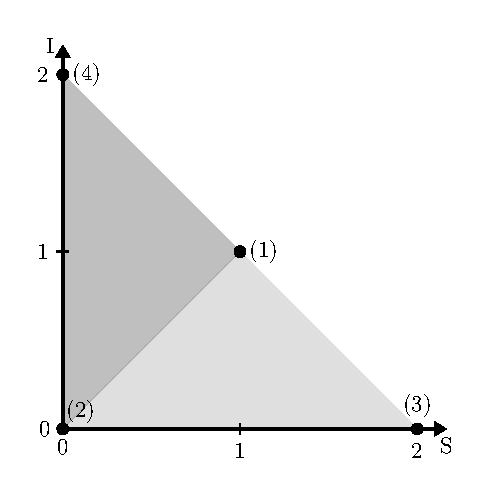
\includegraphics[scale=0.65]{graphics/presentation_qm.pdf}\,\cite{Tegmark_15_long}
			\footnotesize
			(1): $\rho = \frac{1}{2} \del{\ketup\!\braup + \ketdown\!\bradown}$\\
			\hspace{-1.65cm}(2): $\rho = \ketup\!\braup$\\
			\hspace{-.2cm}(3): $\rho = \frac{1}{4} (\ketup\!\braup + \ketdown\!\braup$\\\qquad\qquad $+ \ketup\!\bradown + \ketdown\!\bradown)$\\
			(4): $\rho = \frac{1}{2} \del{\ketup\!\ketup + \ketdown\!\ketdown}$ \\\qquad\qquad$\del{\braup\!\braup + \bradown\!\bradown} $\\
		\end{column}		
	\end{columns}
\end{frame}